\documentclass[AutoFakeBold,zihao=-4]{ctexart}

\usepackage{geometry}
\usepackage{graphicx}
\usepackage{amsmath}
\usepackage{bm}
\usepackage[ruled,linesnumbered]{algorithm2e}
\usepackage{multicol}
\usepackage{float}
\usepackage{cite}

\graphicspath{{image/}}

\geometry{a4paper,left=2cm,right=2cm,top=2.5cm,bottom=2cm}

\renewcommand{\baselinestretch}{1.2}
\renewcommand{\algorithmcfname}{算法}
\newenvironment{sequation}{\begin{equation}\small}{\end{equation}}
\newenvironment{sequation*}{\begin{equation*}\small}{\end{equation*}}
\newenvironment{subsequations}{\begin{subequations}\small}{\end{subequations}}

\bibliographystyle{ieeetr}

\ctexset{
	section = {
		name = {第,章},
		format += \heiti \zihao{-3},
		number = \chinese{section},
	},
	subsection = {
		format += \heiti \zihao{4},
	},
	subsubsection = {
		format += \heiti \zihao{-4},
	},
}

\title{\songti \bfseries \zihao{3} 对三维模型采集的视觉传感器设计规划}
\author{S. Y. Chen, Y. F. Li}
\date{}

\begin{document}
	\maketitle
	\textit{\songti \bfseries 摘要}
	
	本文提出了一种通过主动视觉系统来自动获取未知物体三维模型的新型设计,其中视觉传感器围绕目标从一个视点移动到下一个视点,以获得其完整的模型。在每个步骤中,自动确定传感参数,以逐步建立三维目标模型。该方法是通过分析目标的表面趋势来开发的,趋势面是一个曲面的区域特征,用于描述全局的变化趋势。以往的趋势分析方法通常关注点在于生成多项式方程来解释三维的回归曲面,而本文提出了一种新的数学模型来预测目标曲面的未知区域。通过分析曲面曲率,建立了统一曲面模型。此外,定义了一个确定探索方向的准则,并开发了一种确定下一个视图参数的算法。对该方法进行了实现,验证了所提出的方法。
	
	\textit{\songti \bfseries 索引术语}
	
	模型采集、传感器放置、曲面预测、三维建模、趋势曲面、视点规划、视觉传感器。

	\section{引言}
	使用机器视觉来获得物体的三维模型对许多实际应用来说是非常重要的。在这样的任务中,当没有物体或环境的事先信息时,我们希望能够在运行时自动生成一个多视点规划.视点或传感器的位置需要在满足放置约束条件,例如焦点,视场,遮挡和避免碰撞的同时,能够预测被测物体不可视的部分。这样的策略确定了后续的优势点,这样的好处在于减少甚至消除了人工操作,否则,为了观测物体的表面特征,手工操作是不可避免的。没有视点规划的系统通常必须利用多达数十个范围图像来完成一项典型任务,并且它们之间存在明显的重叠。
	
	关于通过移动视觉传感器进行物体建模的研究\cite{allen20033d}已经持续了十几年。自1988年Cowan和Kovesi\cite{cowan1988automatic}在这方面进行了早期的尝试后,已有许多关于传感器布局或视点规划的作品发表。早期的工作主要集中在传感器建模、传感器的光学和几何参数分析以及传感器位置约束等方面。后来,利用计算机辅助设计(CAD)模型,在基于视觉的检测和物体识别方面也进行了相关应用的研究。“生成-测试”法和综合法是该阶段探讨的主要课题。
	
	虽然对优化于基于模型的传感器放置来说是必要的\cite{chen2004automatic},而在对许多使用机器视觉的任务中是很重要的一环:对于未知物体或环境的视点规划中,这却是一个问题。报道的这方面的研究工作成果离实际应用还很遥远。在这个问题上所进行的大部分工作主要是寻找最佳的视图来对一个物体进行数字化处理,并且在不会出现缺失区的情况下,使得视图的数量尽可能的少。例如,Papdopoulos-Orfanos和Schmitt\cite{papadopoulos1997automatic}利用体积表示法,研究了窄视场范围扫描仪的次佳视图问题的解决方案。他们的工作重点是避免碰撞,因为小视场使得传感器紧贴物体导航。
	
	在以往的建模方法中, “遮挡”和不确定性与视点规划有很强的关联性, Kutulakos等人\cite{kutulakos1995global}利用感知表面与传感器位置的边界变化来复原形状. Kutulakos等人\cite{kutulakos1995global}利用传感表面与遮挡之间的边界变化与传感器位置的关系来恢复形状。Maver和Bajcsy\cite{maver1993occlusions}也使用了类似的基于直方图的技术,来寻找能够照亮从遮挡区域衍生出的最边缘特征的观察向量。Whaite和Ferrie\cite{whaite1997autonomous}使用传感器模型,通过射线投射来评估成像过程在一组离散方向上的功效:让能最好地改善模型的传感器方向被选择用于下一次成像。Pito\cite{pito1999solution}的工作通过确定能够改进当前模型的位置子集,消除了从每个可能的传感器位置进行射线投射的需要。研究了一种不确定性驱动的方法\cite{li2005information},以最大化下一个视图的信息增益。
	
	在增量物体建模的下一个最佳视角(next best view,NBV)问题上,Zha等\cite{zha1997active}解决了确定下一个最佳视角的两个主要问题:1)球面空间的统一镶嵌及其在二维阵列上的映射;2)由评估视角作为NBV的增量更新计算。Yu等人\cite{zhien1996next}提出,对于场景中最能观察到的看不见的部分,通过分析前几幅图像得到的平面交点来确定测距传感器的下一个姿态。他们在场景周围设置了一个球体,然后选择下一个视角,给出最大的未观察区域。Pito等\cite{pito1999solution},\cite{pito1996sensor}提出了在未知部分数字化过程中规划范围相机的解决方案。Arbel等人\cite{arbel1999viewpoint}展示了如何利用熵图引导主动观察者沿着最佳轨迹前进,以及如何利用熵最小化作为选择下一个最佳视图的基础来制定凝视规划策略。在\cite{banta1996autonomous}中,Banta和Abidi描述了一个系统,在理想情况下,NBV将揭示最大数量的先前未知的场景信息。Reed等人\cite{reed2000constraint}确定了能见度体积,即传感器对特定目标的无遮挡视野内的空间体积。在\cite{marchand1997active}和\cite{marchand1999active}中,假设场景只由多面体物体和圆柱体组成。提出的解决NBV问题的技术是深度优先搜索算法,该策略保证了场景重建的完整性。
	
	视点规划中要考虑的另一个因素是必须满足的约束条件。为此,有两种不同的方法被广泛使用:加权函数法和棋盘空间法。前者\cite{reed2000constraint},\cite{tarabanis1995mvp,triggs1995automatic,gu1999robust,cowan1989determining,tarabanis1995survey}采用了一个函数,将代表位置约束的几个分量结合起来。这种方法通常用于基于模型的规划任务中\cite{trucco1997model}。后一种方法\cite{pito1999solution,li2005information,zha1997active},\cite{morooka1999computations},\cite{wong1999next}主要用于对象建模任务。它将待建模对象周围的球体或圆柱体进行镶嵌,产生一个视点空间或查找阵列\cite{morooka1999computations}。物体表面被分割为虚空表面、可见表面、不可见表面和不确定表面。工作空间也被划分为虚空体积和观察体积。然后制定一个算法来规划一个视点序列,这样就可以对整个物体进行采样。这种方法对于处理一些小而简单的物体是有效的,但对于大而复杂的物体,如有许多凹面的环境,由于不能解决遮挡约束问题,所以很难建模。
	
	因此,以往的工作往往是以体积分析或遮挡为指导,寻找最佳下视点,但由于未知目标不存在任何信息,实际上无法给出真正的最佳下视点。虽然传感器布局已经研究了15年以上,也有很多相关的出版物,但大部分的书目都是关于基于模型的任务,例如用于检测或识别。现有的对象建模的传感布局工作通常只针对一些特定的应用。在获取大型物体或环境的表面模型的视图规划方面需要进一步研究。
	
	本文提出了一种使用形状预测的传感器布局的目标驱动方法。我们的方法包括勘探方向的决定和下一个视点的确定。以趋势曲面为线索预测物体的未知部分,利用预测曲面和传感约束确定下一个最佳视点。
	
	\section{增量模型与视点规划}
	
	在三维建模任务中,通常采用增量法来探索物体或环境的未知部分。这就导致了一系列的局部模型采集的查看动作。每一次连续的传感都会给出一些新的信息,这些信息被登记并整合到全局模型中。

	\begin{figure}[h]
		\centering
		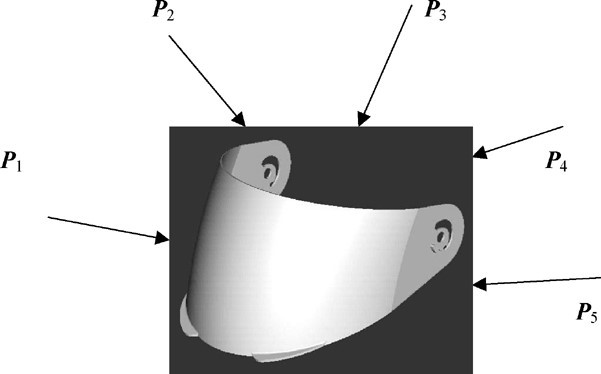
\includegraphics[scale=0.5]{PIC1.jpg}
		\caption{增量模型的多个视点}
		\label{fig-model-point}
	\end{figure}

	在这样的过程中,第一次成像可以设置在任意的一个位置。然后生成一个三维深度图像$ M_{0} $,并注册为初始物体模型$ O_{0} $,接下来,必须确定一个新的观看姿势$ P_{i+1} $,这样建模过程将继续进行,直到整个物体被重建。让前$ i $步(第1步到第i步)重建的全局模型为
	\begin{equation}
		\boldsymbol{M}_{i}=\boldsymbol{M}_{i}(u, v)=(\mathrm{x}(u, v), \mathrm{y}(u, v), \mathrm{z}(u, v))
		\label{eq1}
	\end{equation}
	其中$ u $和$ v $是数字图像上的坐标。使用原点位于视觉传感器中心的坐标系,其Z轴沿观察方向指向,三维深度图像表示为
	
	\begin{equation}
		\mathrm{z}=\boldsymbol{M}_{i}^{\mathrm{w}}(\mathrm{x}, \mathrm{y}), \mathrm{x}, \mathrm{y} \in \mathbf{R}
		\label{eq2}
	\end{equation}

	图\ref{fig-model-point}展示了一个例子,在这个例子中,从$ P_{1} $到$ P_{5} $有五个视点用于获取结构模型。这里的困难是没有关于对象的先验知识。因此,每个连续的视点(从$ P_{2} $到$ P_{5} $)必须在运行时确定。在这样的任务中,传感器放置的关键问题是利用前几步已经建立的部分已知全局模型,确定一个最可行的视点,称为Next-Best-View或Next-Best-Pose\cite{zha1997active}。在这种视觉系统中,必须开发传感器位置或视点规划的算法,以动态确定传感器的位置、方向和光学设置。本文根据已知局部模型的表面趋势确定下一个视点。
	
	\section{用于模型预测的趋势面}
	\subsection{趋势分析}
	曲面趋势描述的是曲面的全局形状。趋势曲面分析是一种处理空间数据的全局方法。从数学上讲,一个映射的曲面可以分成两个部分--趋势的趋势和趋势的残差。趋势是一个曲面的特征,而残差是局部波动(空间频率高),是非全局性的。(图\ref{fig-trend})
	
	\begin{figure*}[h]
		\centering
		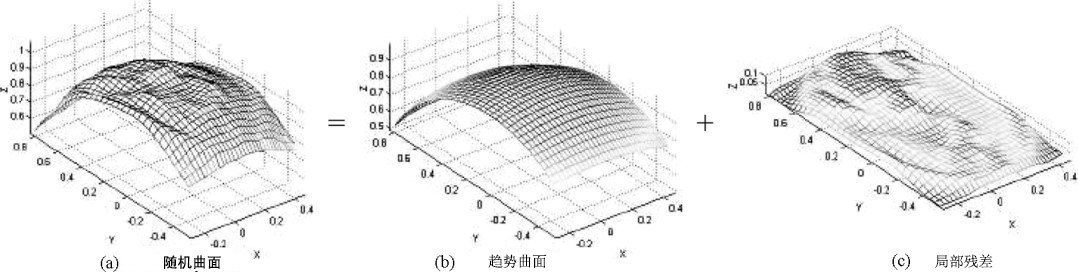
\includegraphics[scale=0.5]{PIC2}
		\caption{ 趋势是表面的区域特征}
		\label{fig-trend}
	\end{figure*}

	趋势曲面分析常用于三维空间的拟合和插值回归曲面,作为面积数据的平滑表示。假设某一特定现象的空间分布可以用某种形式的连续曲面来表示,通常是一个确定的几何函数。观测到的空间格局可以看作是这样一个曲面和一个“随机的”,或是说局部 变量的总和。该曲面是两个正交坐标轴的函数,可以用以下方法表示。
	\begin{equation}
		z=f(x, y)+e
		\label{eq3}
	\end{equation}
	其中点$ (x,y) $的变量$ z $是坐标轴的函数,加上误差项$ e $。这个表达式是通用线性模型(GLM)的广义形式,它是大多数趋势方法的基础。
	
	函数f(x,y)通常被各种项展开或近似,以生成多项式方程。趋势面分析的原理最初是由Agocs\cite{agocs1951least}提出的。为了通过扩展一般线性模型的求和项来发展复杂的、平滑的地球物理数据方程,Krumbein\cite{krumbein1959sorting}定义了标准多元回归分析和趋势方法之间的关系。一个n阶的三维曲面可以用幂级数列给出为
	\begin{equation}
		f(u, v)=\sum_{i=0}^{n} \sum_{j=0}^{i} b_{\mathrm{ij}} u^{j} v^{i-j}
		\label{eq4}
	\end{equation}
	其中$ u $和$ v $是任意正交参考系上的坐标,$ b_{ij} $是曲面的常数系数($ b_{00} $为曲面基数)。
	
	趋势部分对于预测物体或环境中未被看到的部分很有用,因此在本研究中用于确定下一个视点。残差(局部特征)对视点规划影响不大,但在图像处理过程中应将其过滤掉。
	
	让一个单一曲面$ M $被分割成两部分,$ M_{1} $和$ M_{2} $。
	
	\begin{equation*}
		M=M_{1} \cup M_{2}
	\end{equation*}

	如果表面$ M $变化平稳,则$ M_{1} $和$ M_{2} $的趋势都应与$ M $的趋势大致相等,即:
	
	\begin{equation}
		\text { Trend }(M) \approx \text { Trend }\left(M_{1}\right) \approx \text { Trend }\left(M_{2}\right)
		\label{eq5}
	\end{equation}

	假设视觉方法已经捕捉到了一部分曲面,比如说$ M_{1} $,但是$ M_{2} $仍然未知。那么通过计算$ M_{1} $的曲面趋势,可以预测$ M_{2} $的曲面形状。在本文中,我们将不直接使用(\ref{eq3})或(\ref{eq4})作为表面预测的趋势模型,因为它依赖于解释已知区域的回归。相反,我们将开发一个新的数学模型来描述表面趋势,强调对未知面积的预测。
	
	有了部分已知的模型,就可以根据已知信息决定下一个视图的传感器姿态。这里用两个步骤来做这个决定。第一步是确定探测方向,第二步是根据表面趋势确定传感器姿态。
	
	\subsection{探测方向}
	
	在三维曲面数据采集的每一个连续动作中,只能选择一个方向,称为探测方向,用于规划下一个视点。这个方向需要分三步确定。第一步是检测物体的边界点。它将目标从场景中分割出来,找到那些靠近未知区域但在物体表面的点。第二步,通过评级函数对这些点进行排序。第三步是选择一个评级最高的点来给出探索方向。第一步和第三步可以用简单的方法解决。对于第二步,评级函数描述为
	\begin{equation}
		R(P)=\frac{C_{\mathrm{r}} E^{C e}}{\left(n_{\text {order }}+1\right)^{C n}}
		\label{eq6}
	\end{equation}
	其中$ n_{\text {order }} $为$ P $点的表面阶数,$ E $为$ P $附近未知区域的预期体积,$ C_{r} $、$ C_{n} $、$ C_{e} $为可调系数,可根据应用要求选择。$ C_{n} $体现了新对象信息的权重,$ C_{e} $体现了勘探可靠性的权重。$ C_{r} $为全局比例系数,可设为1,结果$ R (P)$为边界点$ P $的额定值。
	
	以表面阶数(即表面的粗糙度)为主要标准。原因是趋势面可以准确预测表面阶数较低的未知区域。图\ref{fig-exploration}说明了勘探方向的选择标准。
	
	\begin{figure}[h]
		\centering
		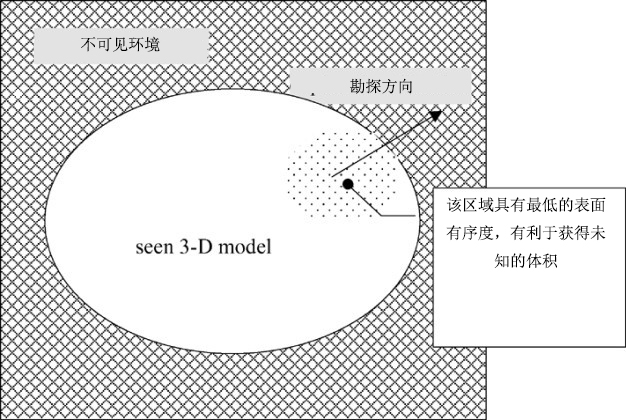
\includegraphics[scale=0.5]{PIC3}
		\caption{对物体表面的探测}
		\label{fig-exploration}
	\end{figure}

	根据(\ref{eq4})定义曲面阶数,其拟合误差相同。为了避免曲面拟合的计算,我们可以近似地计算小范围内曲率的积分值,即:
	\begin{equation}
		n_{\text {order }}(u, v) \approx \iint_{x, y \in S(u, v)} k_{\min }(x, y) d x d y
		\label{eq7}
	\end{equation}
	其中$ S(x,y) $为点$ (x,y) $的邻域面积。域$ S $的面积大小取决于传感器的视场(FOV),例如,用$ 20 \times 20 \mathrm{~mm}^{2} $或$ 30 \times 30 $像素.$ k_{\min }(x, y) $是点$ (x,y) $沿特定方向的曲率。
	
	只需计算已知曲面边界附近区域的曲面阶数即可,已知模型中心区域的曲面阶数不影响探测方向。在得到最小曲面阶数后,即 $ n_{\min }=\min \left\{n_{\text {order }}(u, v)\right\} $,将探测方向设为沿外方向至未知区域。
	
	\subsection{表面预测}
	
	除表面边缘和物体边界外,由于趋势曲面的曲率变化是平稳的,所以通过分析已知曲面的曲率趋势,可以预测物体表面的未知部分。
	
	对于一个曲面点,沿不同的方向有不同的曲率,不过最常用的是主曲率和高斯曲率。为了降低计算复杂度,我们可以只计算沿探索方向的曲线曲率。在不失通用性的前提下,我们可以沿水平方向描述数学公式(否则需要进行坐标变换)。利用平行于x轴的垂直剖面,在y=yv处切开三维曲面,我们得到一条曲面曲线(见图\ref{fig-Curve})。
	
	\begin{figure}[h]
		\centering
		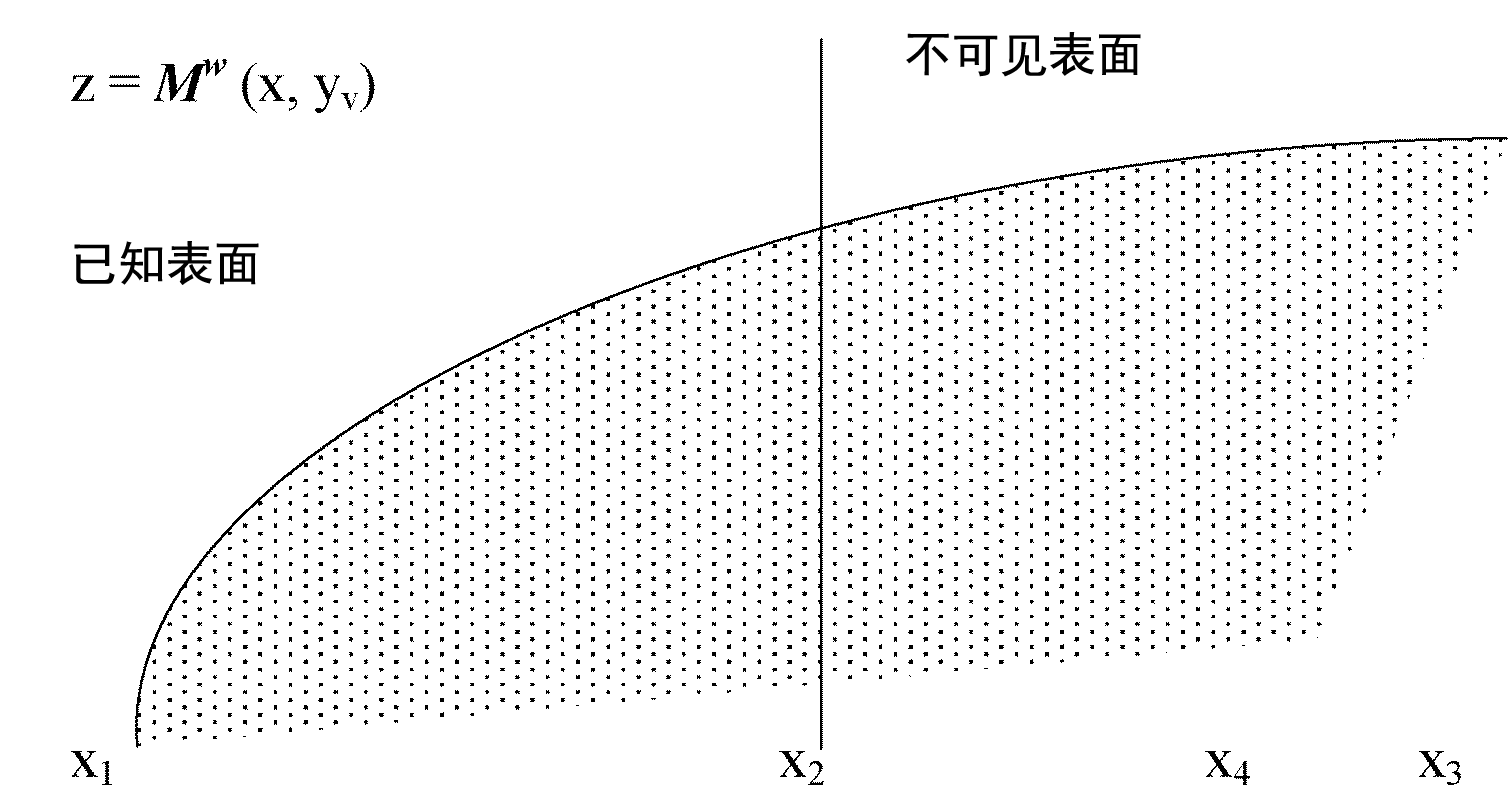
\includegraphics[scale=0.2]{PIC4}
		\caption{剖面图上的曲线}
		\label{fig-Curve}
	\end{figure}

	\begin{equation}
		z_{v}=f_{\mathrm{yv}}(x)
		\label{eq8}
	\end{equation}

	这条曲线的曲率是

	\begin{equation}
		k\left(x, y_{v}\right)=\frac{z_{v}^{\prime \prime}}{\left[1+\left(z_{v}^{\prime}\right)^{2}\right]^{3 / 2}}
		\label{eq9}
	\end{equation}

	设$ X_{\mathrm{k}}=\left[x_{1}, x_{2}\right] $为曲面曲线已知部分的域。为了预测不可见曲面,我们用$ x $对$ k $进行线性回归,得到拟合曲线$ c_{v} $,用于逼近曲线$ z_{v} $上的曲率趋势。因此
	\begin{equation}
		c_{v}(x)=a x+b, x \in\left[x_{1}, x_{3}\right]
		\label{eq10}
	\end{equation}
	其中[x1,x3]为整个域,包括已知面积和未知面积,即$ \left[x_{1}, x_{3}\right]=\left[x_{1}, x_{2}\right] \cup\left[x_{2}, x_{3}\right] $。两个参数a和b由表面曲线的已知部分拟合确定,即:
	\begin{equation}
		a=\frac{6\left(x_{2}+x_{1}\right) \int_{x 1}^{x 2} k\left(x, y_{v}\right) d x-12 \int_{x 1}^{x 2} x k\left(x, y_{v}\right) d x}{\left(x_{1}-x_{2}\right)^{3}}
		\label{eq11}
	\end{equation}
	和
	\begin{equation}
		b=\frac{\left[\int_{x 1}^{x 2} k\left(x, y_{v}\right) d x-\frac{1}{2}\left(x_{2}^{2}-x_{1}^{2}\right) a\right]}{\left(x_{2}-x_{1}\right)} .
		\label{eq12}
	\end{equation}

	不可见区域的曲率预计为
	\begin{equation}
		c_{v}=\left\{\begin{array}{ll}
			a x+b, & k\left(x, y_{v}\right)<k_{\max } \\
			k_{\max }, & k\left(x, y_{v}\right) \geq k_{\max }
		\end{array}, x \in\left[x_{2}, x_{4}\right]\right.
		\label{eq13}
	\end{equation}
	其中$ x_{2}<x_{4}<x_{3} $是满足约束条件的域,即物体表面将在传感器的FOV中。$ k_{max} $是限制最大曲率的给定阈值。它可以设置在[1,20]/感应距离(1/mm)的范围内的一个值。那么,物体未被看到的部分的表面曲线将是下式的解
	
	\begin{equation}
		\frac{\left\|z^{\prime \prime}\right\|}{\left[1+\left(z^{\prime}\right)^{2}\right]^{3 / 2}}-c_{v}=0
		\label{eq14}
	\end{equation}

	这个微分方程的解是
	\begin{equation}
		z=\pm \int \frac{\left(a x^{2}+2 b x+2 C_{1}\right)}{\sqrt{4-\left(a x^{2}+2 b x+2 C_{1}\right)^{2}}} d x+C_{2}, x<\frac{\left(k_{\max }-b\right)}{a}
		\label{eq15}
	\end{equation}
	或
	\begin{equation}
		z=\pm \sqrt{k_{\max }^{2}-\left(x-C_{3}\right)^{2}}+C_{4}, x \geq \frac{\left(k_{\max }-b\right)}{a}
		\label{eq16}
	\end{equation}
	其中$ C_{i}(\mathrm{i}=1,2,3,4) $为微分常数,可根据边界条件确定,如$ z\left(x_{2}\right)=z_{2} $和$ z^{\prime}\left(x_{2}\right)=z_{2}^{\prime} $。符号“+”或“-”也可以根据表面曲线的已知部分(凸或凹)来确定。由于预测曲线是根据已知面积的趋势分析得出的,所以称为趋势曲线。
	
	\section{视点规划}
	\subsection{放置参数}
	在传感器放置问题中,我们需要指定传感器的放置参数\cite{chen2004automatic}。这里的放置参数包括传感器的位置$ \left(x_{p}, y_{p}, z_{p}\right) $和方向$ (\alpha, \beta, \gamma) $。安置约束条件可以包括可见度、焦点、视场、视角、分辨率、重叠、遮挡,以及一些操作约束条件,如传感器姿势的运动可达性和机器人与环境的碰撞。设分辨率约束为
	
	\begin{equation}
		r_{p}=2 \sqrt{\left(x_{p}-x_{2}\right)^{2}+\left[z_{p}-z\left(x_{2}, y_{v}\right)\right]^{2}} \frac{\tan \left(\frac{\Omega}{2}\right)}{N}<r_{\max }
		\label{eq17}
	\end{equation}
	其中$ N $是数字图像扫描线上的像素数,$ \Omega $是传感器的视角。公式(\ref{eq17})描述了图像上的一个像素与其在物体表面的实际大小之间的关系。
	
	为了满足传感器位置对分辨率和FOV的约束,通过搜索算法确定(\ref{eq13})中的参数$ x_{4} $。那么趋势曲线的中点为
	
	\begin{equation}
		Q_{\mathrm{yv}}=\left(x_{v}, y_{v}, z_{m v}\right), z_{m v}=f\left(x_{v}, y_{v}\right), x_{v}=\frac{x_{2}+x_{4}}{2}
		\label{eq18}
	\end{equation}

	通过将截面平面移动到不同的位置,在$ -Y_{\mathrm{fov}}<y_{v}<Y_{\mathrm{fov}} $的域内,我们得到一系列的表面趋势曲线。将每一条这样的曲线的中点连接起来,我们就可以得到一条新的曲线
	\begin{equation}
		L_{i+1}=L\left(Q_{\mathrm{yv}}\right),-Y_{\mathrm{fov}}<y_{v}<Y_{\mathrm{fov}}
		\label{eq19}
	\end{equation}
	其中$ L $为曲线函数,$ (i+1) $表示下一个视图姿态。
	
	计算中心点,得到参考点的位置(即新的场景中心):
	\begin{equation}
		O_{i+1}=\left(x_{i+1}^{o}, y_{i+1}^{o}, z_{i+1}^{o}\right)
		\label{eq20}
	\end{equation}
	其中,$ x_{i+1}^{o}=\int_{L_{i+1}} x L d l / \int_{L_{i+1}} L d l, \quad y_{i+1}^{o} \quad= \int_{L_{i+1}} y L d l / \int_{L_{i+1}} L d l,  z_{i+1}^{o}=\int_{L_{i+1}} z L d l / \int_{L_{i+1}} L d l $。
	
	
	现在可以确定传感器的位置和观察方向。为了达到最大的观察角度(即观察方向与表面切线之间的角度),以最小化重建不确定度,观察方向选择为预测表面平均法线的倒数,也就是
	\begin{equation}
		\begin{aligned}
			V_{i+1} &=-\frac{\iint N(x, y) d x d y}{\iint d x d y}\\
			&=-\frac{\iint(\mu \mathbf{i}, \nu \mathbf{j}, \kappa \mathbf{k})(x, y) d x d y}{\iint d x d y}\\
			&=\left(-\mu_{i+1} i,-\nu_{i+1} j,-\kappa_{i+1} k\right)
		\end{aligned}
		\label{eq21}
	\end{equation}
	其中,$ \mu(x, y)=\partial f / \partial x, \nu(x, y)=\partial f / \partial y, \kappa(x, y)=-1 $,$ N(x,y) $为点$ (x,y,z) $上的曲面法线。
	
	下一个视点的传感器位置$ P_{i+1}=\left(x_{i+1}^{\mathrm{p}}, y_{i+1}^{\mathrm{p}}, z_{i+1}^{\mathrm{p}}\right) $规划为以下方程组的解:
	\begin{equation}
		\left\{\begin{array}{l}
			\frac{x_{i+1}^{o}-x_{\imath+1}^{\mathrm{p}}}{\prod O_{i_{i}+1}-P_{i+1} \|_{2}}=\frac{-\mu_{n+1}}{\left\|V_{i+1}\right\|_{2}} \\
			\frac{y_{i+1}^{o} y_{i+1}^{\mathrm{p}}}{\left\|O_{i+1}-P_{i+1}\right\|_{2}}=\frac{-\nu_{i+1}}{\left\|_{i+1}\right\|_{2}} \\
			\left\|O_{i+1}-P_{i+1}\right\|_{2}-\frac{r_{\max } N}{2 \tan \frac{\Omega}{2}}=c_{c m p}, \quad c_{c m p} \geq 0
		\end{array}\right.
		\label{eq22}
	\end{equation}
	其中,$ c_{cmp} $是一个正常数,用于补偿深度值范围。$ \Omega $是传感器的视角,$ \left\|V_{i+1}\right\|_{2}=\sqrt{\mu_{i+1}^{2}}+\nu_{i+1}^{2}+\kappa_{i+1}^{2}$,$ \left\|O_{i+1}-P_{i+1}\right\|_{2} $位于区间$ O_{i+1} $到$ P_{i+1} $。
	
	\subsection{布局算法}
	主动式传感器放置的算法总结如下
	\begin{algorithm}
		\caption{确定放置参数的算法}
		\label{ag1}
		根据初始视图或前向视图得到的三维曲面或局部模型,找到确定勘探方向的边界位置\;
		对于每个候选位置,计算其表面阶数和预期未知体积。然后选择一个勘探方向,该方向由评级函数(\ref{eq7})决定\;
		通过勘探方向,计算出所选位置的表面趋势或曲线趋势\;
		通过公式(\ref{eq11})和(\ref{eq12})确定常数$ a $和$ b $\;
		确定(\ref{eq15})和(\ref{eq16})中$ C_{z} $的值和$ z $的符号\;
		通过算法\ref{ag1}确定$ x_{4} $的值\;
		通过公式(\ref{eq18})确定每条趋势曲线的中点\;
		通过公式(\ref{eq20})确定场景中心\;
		通过公式(\ref{eq21})确定视角方向\;
		通过公式(\ref{eq22})确定视点位置\;
	\end{algorithm}
	
	使用这种方法,传感器的方向确定为垂直向下观察预测的物体表面。确定与物体的距离,使其能够获取未知表面的最大体积,同时满足一些约束条件,如分辨率和FOV。最后,视觉传感器的放置参数以矢量形式给出:
	\begin{equation}
		\boldsymbol{S}_{i+1}=\left(x_{i+1}^{P}, y_{i+1}^{P}, z_{i+1}^{P}, \mu_{i+1}, \nu_{i+1}, \kappa_{i+1}\right)
		\label{eq23}
	\end{equation}
	这个放置向量是基于局部坐标系的,它需要通过乘以变换矩阵转换到全局坐标系。
	
	\subsection{建模过程}
	
	最后,迭代建模过程如图5所示,图中符号$ \mathrm{Si}(\mathrm{i}=1,2, \ldots, 7) $分别代表的状态为:
	\begin{figure}[h]
		\centering
		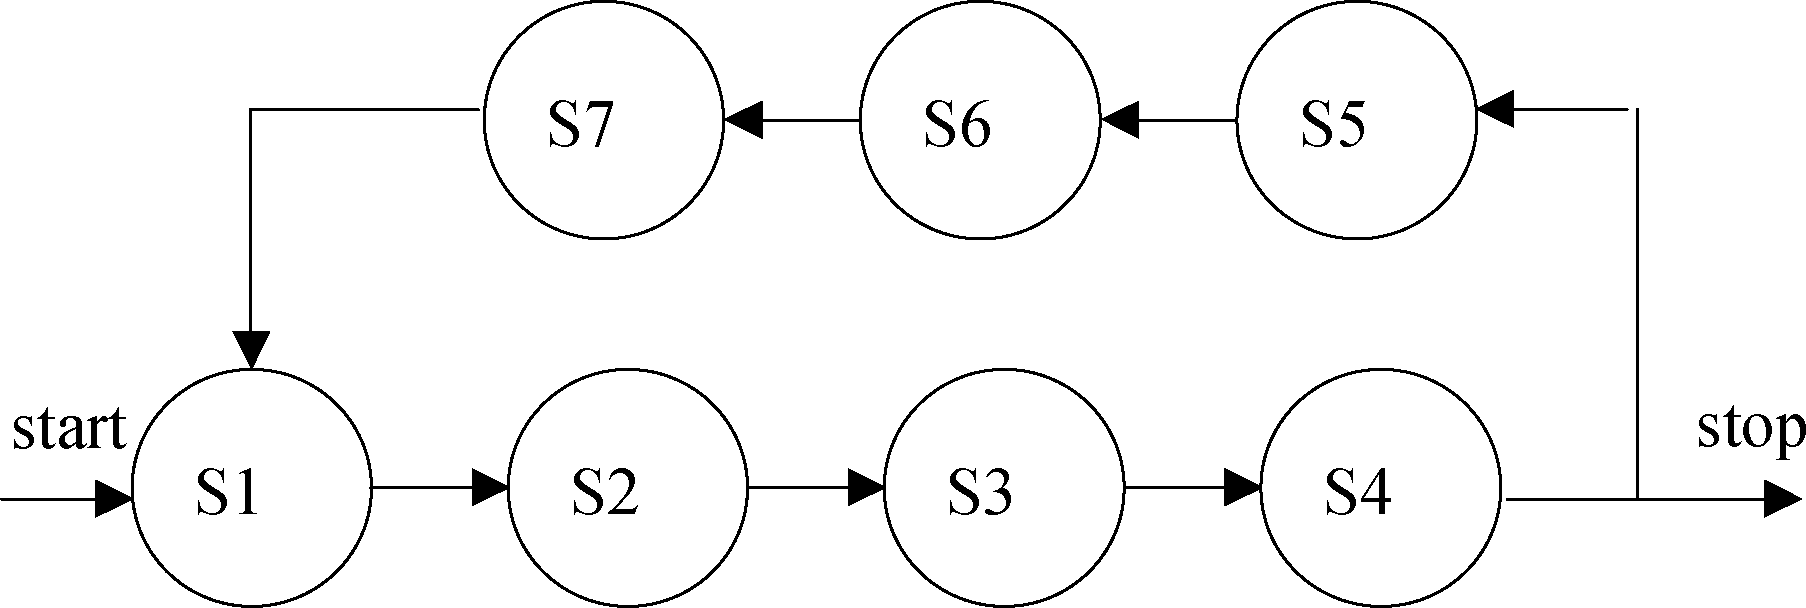
\includegraphics[scale=0.15]{PIC5}
		\caption{建模过程}
		\label{fig-Modeling-process}
	\end{figure}
	\begin{enumerate}
		\item[S1)] 视点的获取
		\item[S2)] 三维局部模型的重建
		\item[S3)] 注册并与全局模型融合
		\item[S4)] 模型分析和完成情况检查
		\item[S5)] 勘探方向选择的排序
		\item[S6)] 计算趋势面并确定下一个视图
		\item[S7)] 将机器移动到新的视点
	\end{enumerate}
	由于表面数据集(三角网格或点云)来自不同的视点,因此有必要将它们与S3中的全局模型进行注册和融合。采用分割和合并算法来执行这样的注册和融合过程。S4中的终止条件是根据模型完成准则确定的。在实施中,已知的局部模型表面被分割成一组小区域。定义了未知孔,它是没有数据的区域,但既不在已知的空卷中,也不指向不可到达的空间。然后,一个算法检测小区域附近的未知孔(不确定区域),并估计其大小。如果未知孔的直径大于一定的值$ d_{h} $(如10mm),这取决于应用,则应规划一个新的视点。否则,重建过程将终止。$ d_{h} $的选择会影响视图总数、表面质量和模型的完整性。小$ d_{h} $有利于获得完整的物体模型,但会增加视图数量,从而增加获取成本。
	
	\section{误差分析}
	需要注意的是,趋势所预测的曲面只是可能的曲面形状。这里分析所产生的误差是在假设实际曲面是由典型的一阶或二阶曲线组成的情况下进行的。我们首先定义一个预测误差。绝对预测误差定义为预期曲面与实际物体曲面之差,即:
	\begin{equation}
		E=\iint_{M_{i+1}}\left\|z(x, y)-z_{\exp }(x, y)\right\| d x d y
		\label{eq24}
	\end{equation}
	其中$ M_{i+1} $是下一个视图要观察的场景的域。相对误差定义为:
	\begin{equation}
		E^{r}=\iint_{M_{i+1}}\left\|\frac{z(x, y)-z_{\exp }(x, y)}{z(x, y)}\right\| d x d y \times 100 \%
		\label{eq25}
	\end{equation}
	由于曲面曲线的形状是在截面平面上计算出来的,所以我们只需要在二维坐标系上分析一、二阶曲线,即直线、圆曲线、抛物线、椭圆曲线和双曲线的误差。这些曲线在实际工业设计中应用广泛,大多数物体表面都可以分解为这些曲线。由于曲线的原点位置不影响物体表面的曲率,所以不需要考虑曲线的原点位置。因此我们总是让曲线的原点为(0,0)。

	对于一条直线,例如$ z=c_{1} x+c_{2} $,根据(\ref{eq11})和(\ref{eq12}),我们有$ a=0 $和$ b =0 $。参考(\ref{eq15}),发现预测的曲线函数$ z_{p}(x) $与实际曲线函数相同。因此预测直线的误差为
	\begin{equation*}
		E_{\text {line }}=\int_{x_{2}}^{x_{4}}\left\|z-z_{\text {exp }}\right\| d x=0
	\end{equation*}

	同理,对于圆曲线$ z=\sqrt{R^{2}-x^{2}} $,我们也可以得到$ E_{\text {circle }} \equiv 0 $,这意味着如果物体表面是由圆曲线或直线曲线组成,那么预测表面与实际表面之间没有误差。因此,我们可以准确地将视觉传感器放置在下一个视图姿势中,以感知最大的信息。示例对象包括任意姿势下的立方体和球,以及限制姿态下的圆柱体和圆锥体。
	
	一些典型的二阶曲线如下:
	\begin{equation*}
		\begin{aligned}
			\text { 抛物线 }: z &=A_{0} x^{2} \\
			\text { 椭圆 }: z &=\frac{1}{B_{0}} \sqrt{1-A_{0}^{2} x^{2}} \\
			\text { 双曲线 }: z &=\frac{1}{B_{0}} \sqrt{1+A_{0}^{2} x^{2}}
		\end{aligned}
	\end{equation*}

	由于(\ref{eq11})在$ a \neq 0 $和$ b \neq 0 $时是不可积的,对于这三条曲线,用二阶泰勒多项式函数来逼近它。即
	\begin{equation*}
		z_{p}(x+\Delta)=z_{p}(x)+z_{p}^{\prime}(x) \Delta+\frac{1}{2} z_{p}^{\prime \prime}(x) \Delta^{2}+R_{3} \Delta^{3}
	\end{equation*}
	其中
	\begin{equation*}
		\begin{array}{l}
			z_{p}^{\prime}=\frac{\left(a x^{2}+2 b x+2 C_{1}\right)}{\sqrt{4-\left(a x^{2}+2 b x+2 C_{1}\right)^{2}}},  \\
			z_{p}^{\prime \prime}=\frac{8(a x+b)}{\left[4-\left(a x^{2}+2 b x+2 C_{1}\right)^{2}\right]^{3 / 2}}
		\end{array}
	\end{equation*}

	在实际实施过程中,由于$ \Delta \ll 1 $ 且 $ R_{3} \Delta^{3} \approx 0 $,$ R_{3} \Delta^{3} $项实际上是被忽略的,因此预测曲线可以用数值计算。变量a和b根据(\ref{eq11})和(\ref{eq12})确定。常数$ C_{1} $的确定还要考虑边界条件$ z_{p}^{\prime}\left(x_{2}\right)=z^{\prime}\left(x_{2}\right) $,即
	\begin{equation}
		C_{1}=\frac{z^{\prime}\left(x_{2}\right)}{\sqrt{\left[z^{\prime}\left(x_{2}\right)\right]^{2}+1}}-\frac{1}{2} a x_{2}^{2}-b x_{2}
		\label{eq26}
	\end{equation}

	然后,通过实际值$ z $与预测值$ z $的方差来确定这些曲线的绝对误差和相对误差。进行了仿真,对$ a,b,C_{1} $,观察了抛物线、椭圆、双曲线、圆的绝对误差和相对误差的结果,假设$ A_{0}=1, B_{0}=0.5 $。作为对算法的验证,结果表明,如果实际曲线是圆的一部分,预测误差始终为零,即$ a=0, b=1, C_{1}=0, E_{circle}=0 $。结果也表明,预测其他二阶曲线的误差非常小(相对误差在$ 10^{-7} $级)。因此,我们可以准确地将视觉传感器放置在下一个视图姿势中,以观察由这种表面组成的物体,当使用均匀表面趋势模型(\ref{eq15})预测的预期曲线。但是,对于每条不同的曲线,常数($ a, b$和$ C_{1} $)是不同的,它们应该根据曲线的已知部分动态地确定。
	
	\section{实验}
	\subsection{实施方面的考虑}
	为了在实际系统中实现所提出的方法,我们必须考虑许多其他因素和条件。事实上,本方法必须与其他技术和算法相结合,实现建模过程的自动化,如图\ref{fig-Modeling-process}所示。在此条件下,对所提出的方法的评价就变得很困难,目前我们只能提供一些简单的例子,在建模过程中,有少量的人为干扰。
	
	必须注意的一个问题是噪声滤波。由于物体表面的曲率对噪声很敏感,而三维图像的局部特征对表面趋势影响不大,所以对图像应用低通滤波器,这样我们就可以得到一个平滑的表面。当然,对于描述相当大面积形状的趋势,其实对噪声并不敏感。我们也在考虑用一些图像处理的方法来滤除噪声,以更稳定的方式计算形状。
	
	方程(\ref{eq11})和(\ref{eq12})被描述为连续函数。当应用于数字图像处理时,它们可以被写成以下形式
	\begin{subequations}
		\begin{align}
			a &=\frac{m \sum_{i=1}^{m} x_{i} k_{i}-\sum_{i=1}^{m} x_{i} \sum_{i=1}^{m} k_{i}}{m \sum_{i=1}^{m} x_{i}^{2}-\left(\sum_{i=1}^{m} x_{i}\right)^{2}} \tag{\ref{eq11}{a}} \label{eq11a}\\
			b &=\frac{\left(\sum_{i=1}^{m} k_{i}-a \sum_{i=1}^{m} x_{i}\right)}{m} \tag{\ref{eq11}{b}} \label{eq11b}
		\end{align}
	\end{subequations}
	其中$ m $为物体表面已知部分的总点数。
	
	另一个问题是关于曲率的计算。计算物体表面已知部分上各点的曲率,以便确定表面趋势,预测未知部分。但公式\eqref{eq6}不适合用于计算数字图像的曲率,因为计算$ z^{\prime} $和$ z^{\prime \prime} $的误差会很大。在本研究中,我们通过相邻的三个点(三连点),即$ P(x(i-1),z(i-1)), P(x(i),z(i)), P(x(i+1),z(i+1))) $来确定点$ P(x(i),z(i)) $的曲率,每个三连点定义一个圆,曲率$ k(i) $是其半径的倒数。
	
	\subsection{实例}
	
	我们在实验室进行了几次实验,以构建物体模型。本研究中设置的结构光系统获得的范围数据,主要由投影仪和摄像机组成。投影仪为手掌大小的数字投影仪:PLUS U3-1080。 它与计算机相连,通过控制生成一些灰色编码的条纹光模式,用于三维重建\cite{li2003automatic}。CCD相机(PULNIX TMC-9700)有一个1英寸的传感器和一个25mm的镜头。在6DOF机器人(STAUBLI RX-90B)的末端执行器上设计了一个夹具,用于安装结构光系统,其重复性为$ \pm 0.02 \mathrm{~mm} $。这使得三维传感器可以自由移动到工作空间的任意位置。
	\begin{figure}[h]
		\centering
		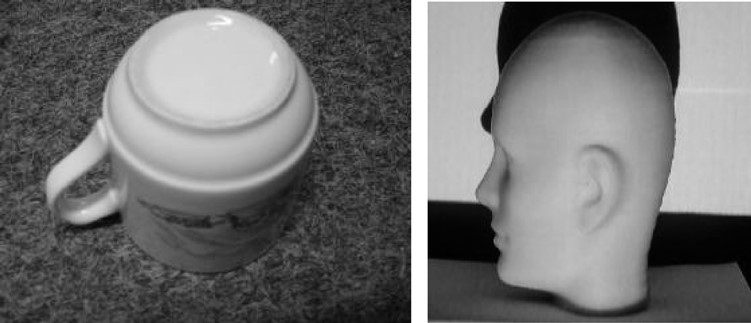
\includegraphics[scale=0.35]{PIC6}
		\caption{要重建的对象}
		\label{fig-Objects}
	\end{figure}

	图\ref{fig-Objects}展示了实验中模型构建的两个对象。在这两种情况下,我们将分辨率约束设置为$ T_{max}=0.85 \mathrm{~mm} $。第一种在这里更详细地演示了程序。它是由四个视图递增建立的。第一个视图被假定为从顶视图中获取。为了确定下一个视图,以获取物体的一些看不见的信息,我们使用趋势曲面法,并开发了一个程序来计算预期曲面曲线。然后计算出趋势,确定下一个视角。
	
	下面展示了第一个对象增量构建中的实验结果,以说明每一步的计算情况。在每一个视图中都获取了一个新的曲面,并将其与现有的曲面整合在一起,形成一个局部模型。勘探方向和传感器位置由提出的方法确定。每个视图的放置参数都设置了一个视点向量,格式为$ [x \quad y \quad z \quad \mathrm{a} \boldsymbol{i} \quad \mathrm{b} \boldsymbol{j} \quad \mathrm{c} \boldsymbol{k}] $,代表三维位置和方向的六个参数。同时,注册向量中还包含了表面积分的六个参数,以便将范围图像转化并注册到一个共同的坐标系中。六个参数中的前三个参数定义了曲面的参考点,另外三个参数通过三轴旋转定义了曲面的方向。这样一来,通过消除重叠/多余的点和缝合非数据区域来改进模型。
	
	\begin{figure}[h]
		\centering
		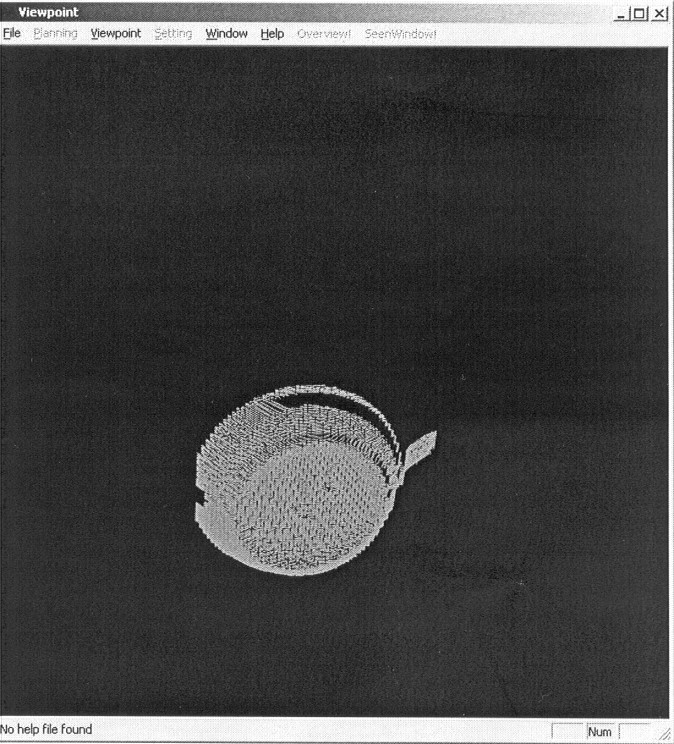
\includegraphics[scale=0.4]{PIC7}
		\caption{从第一视图获得的三维曲面}
		\label{fig-first-view}
	\end{figure}
	第一视图(图\ref{fig-first-view})的对应位置参数为:
	\begin{equation*}
		\begin{aligned}
			\text { Viewpoint }_{1} &=(0,0,457.9333,0,0,-1) \\
			\operatorname{Reg}_{1} &=\mathrm{O}_{\text {global }}=(0,0,0,0,0,0)
		\end{aligned}
	\end{equation*}
	其中视点向量的格式为$ [x \quad y \quad z \quad \mathrm{a} \boldsymbol{i} \quad \mathrm{b} \boldsymbol{j} \quad \mathrm{c} \boldsymbol{k}] $,表示三维位置和方向的六个参数。$ \operatorname{Reg}_{1} $中包含了一些曲面积分的注册参数,这样就可以将范围图像进行变换,并注册到一个共同的坐标系中。六个参数中的前三个参数定义了曲面的参考点,其他三个参数通过三轴旋转定义了曲面的方向。这样一来,通过消除重叠/多余的点和拼接非数据区域来优化模型。
	
	\begin{figure}[h]
		\centering
		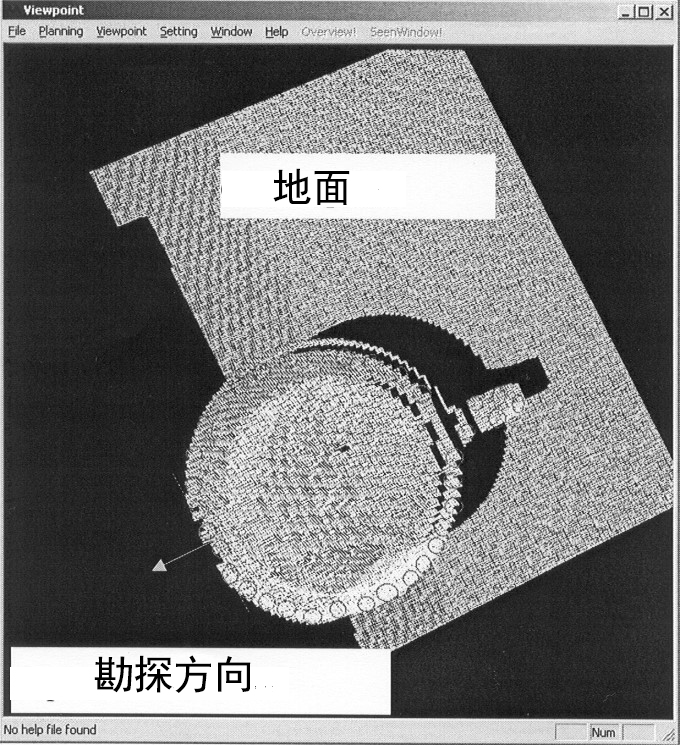
\includegraphics[scale=0.4]{PIC8}
		\caption{被检测为勘探方向的各候选点,根据它们的评级值作出决定}
		\label{fig-Points}
	\end{figure}
	从已知的局部模型中,检测表面边界以找到候选点(图\ref{fig-Points}),并根据\eqref{eq6}进行评级评价,选择一个最佳勘探方向。沿着这个方向,从已知的三维曲面计算出一条趋势曲线(图\ref{fig-Predictive}中虚线红色曲线)。曲线下的空间和地平面被标记为不可到达的空间
	
	\begin{figure}[h]
		\centering
		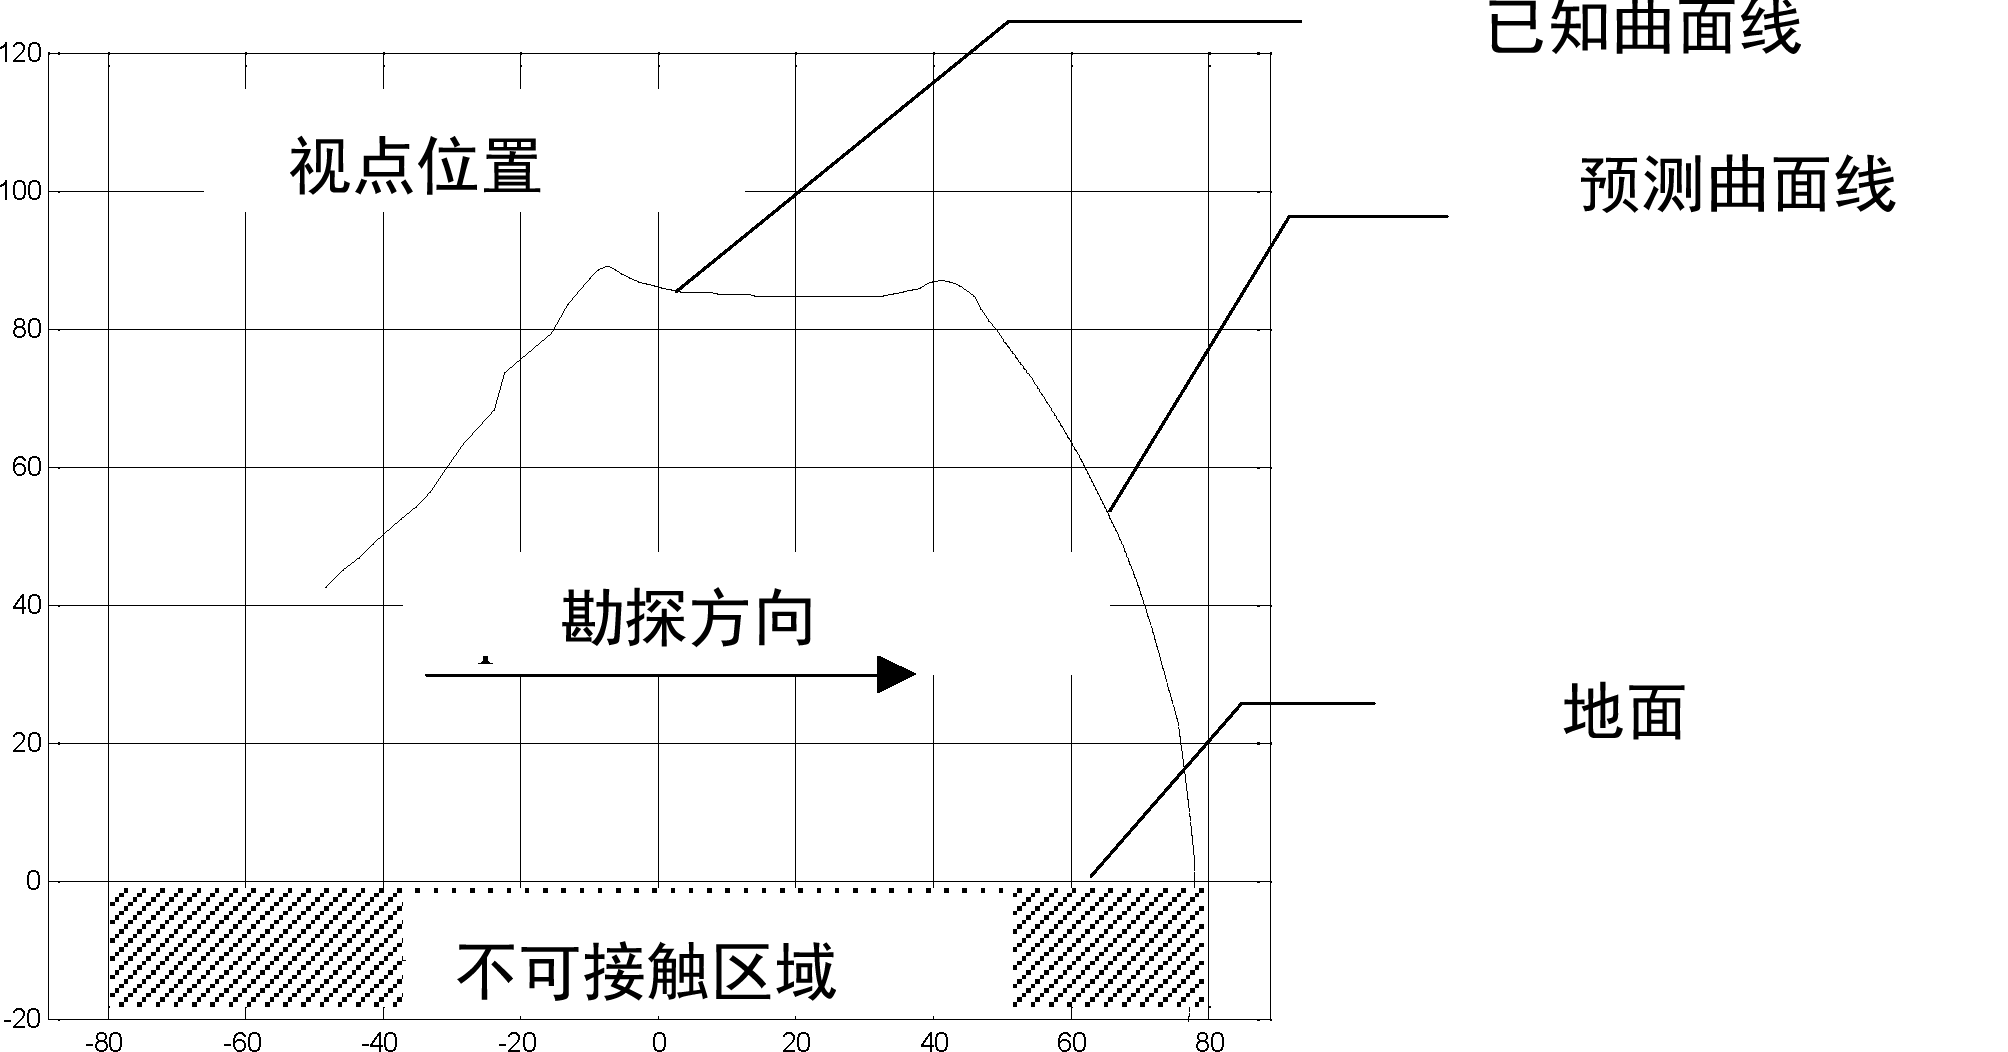
\includegraphics[scale=0.15]{PIC9}
		\caption{预测趋势曲线}
		\label{fig-Predictive}
	\end{figure}

	根据预测的曲线规划传感器的位置和寻找方向。相应的位置参数为
	
	\begin{equation*}
		\begin{aligned}
			&\text { Set\_scene\_center }=[63.9950,-23.0346,40.4942] \\
			&\text { Viewpoint2 }=(502.9636,-26.2364,158.2319\\
			&-0.965838,0.00704474,-0.259052) \\
			&\operatorname{Reg} 2=(-72.06,0.00,40.10,32.01\\
			&-89.89,-30.80)
		\end{aligned}
	\end{equation*}

	与第一步的情况类似,选择候选点,寻找勘探方向。沿着这个方向,计算出几条趋势曲线来预测曲面的未知部分。
	
	传感器的姿势也是根据预测的曲线确定的。相应的放置参数为
	
	\begin{equation*}
		\begin{aligned}
			\text { Set\_scene\_center }&=[-8.485960 .019933 .7807] \\
			\text { Viewpoint3 }&=(21.7862,366.7046,-228.8904\\
			&-0.0747589,-0.757378,0.648683) \\
			\operatorname{Reg} 3&=(30.21,-116.07,40.02,89.83,\\
			&31.10,-89.92)
		\end{aligned}
	\end{equation*}
	
	\begin{figure}[H]
		\centering
		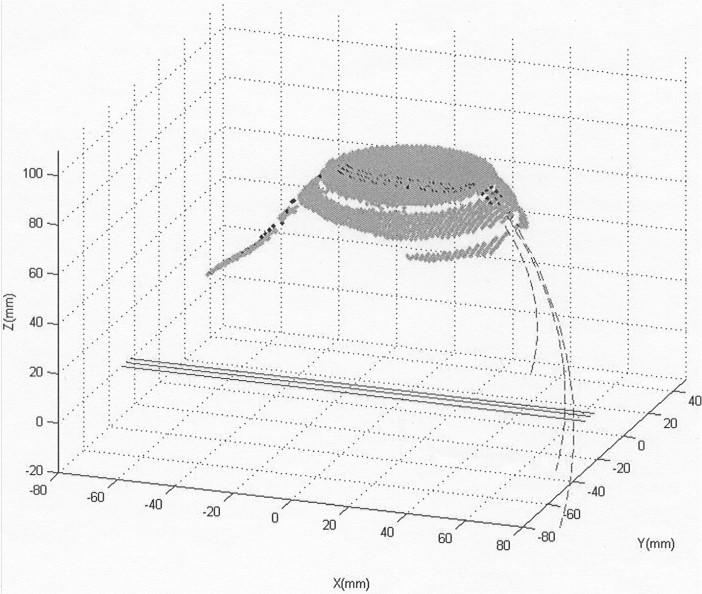
\includegraphics[scale=0.4]{PIC10}
		\caption{得到几条趋势曲线,形成趋势面,从而使下一个观点的决定更加可靠}
		\label{fig-10}
	\end{figure}

	\begin{figure}[H]
		\centering
		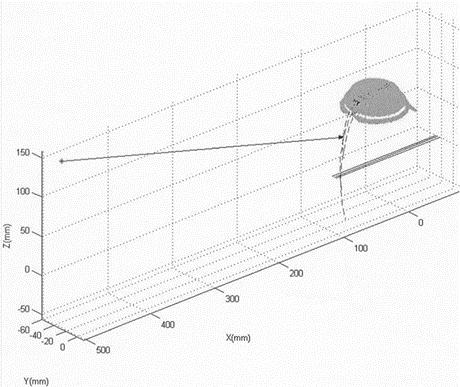
\includegraphics[scale=0.9]{PIC11}
		\caption{规划下一个视点}
		\label{fig-11}
	\end{figure}

	\begin{figure}[H]
		\centering
		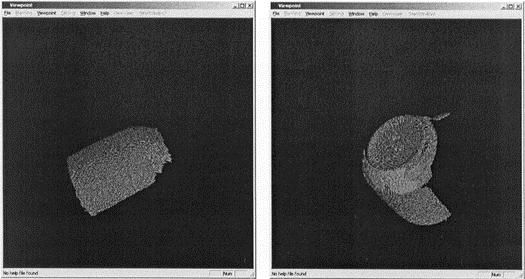
\includegraphics[scale=0.9]{PIC12}
		\caption{从第二视图(左)获得三维曲面,并与第一视图集成,形成物体的部分模型(右)。}
		\label{fig-12}
	\end{figure}

	\begin{figure*}[h]
		\centering
		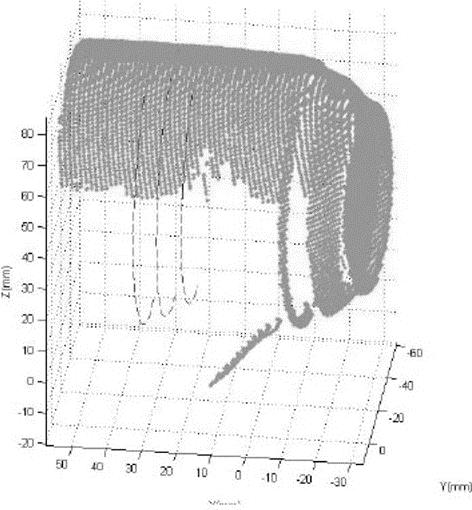
\includegraphics[scale=0.9]{PIC13}
		\caption{第二步的趋势曲线}
		\label{fig-13}
	\end{figure*}

	\begin{figure}[H]
		\centering
		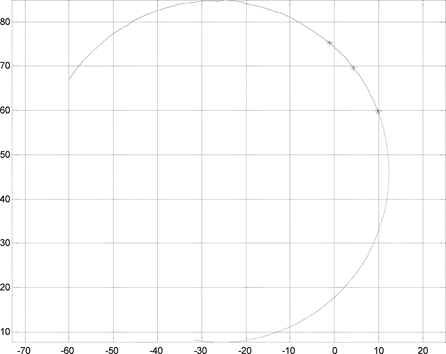
\includegraphics[scale=0.9]{PIC14}
		\caption{ 其中的趋势曲线如图\ref{fig-13}。由于原曲线是圆形的,所以预测非常准确。}
		\label{fig-14}
	\end{figure}

	\begin{figure}[H]
		\centering
		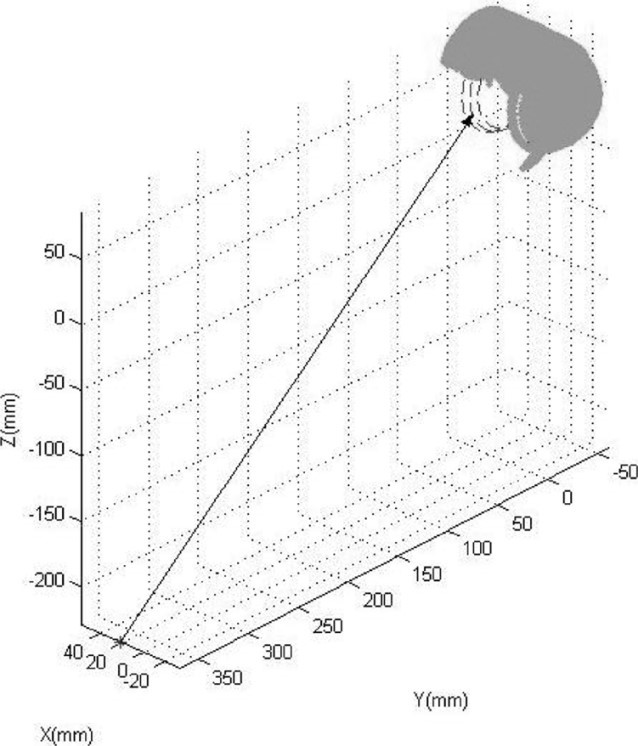
\includegraphics[scale=0.4]{PIC15}
		\caption{下一个视点}
		\label{fig-15}
	\end{figure}
	图\ref{fig-10}至图\ref{fig-15}说明了趋势面的传感决策的两个步骤。对于图\ref{fig-16}中的模型,需要采取进一步的观点决策和曲面采集。这些工作与前面的步骤类似。第四视图的传感器参数确定为(图\ref{fig-17})
	\begin{equation*}
		\begin{aligned}
			\text { Set\_scene\_center }&=[16.3405,-10.1124,35.0603] \\
			\text { Viewpoint } 4&=(15.8901,347.64,-251.11,\\
			&0.0009831,-0.780902,0.624653) \\
			\operatorname{Reg} 4&=(-116.12,-120.01,43.03\\
			&-90.00,22.60,89.31)
		\end{aligned}
	\end{equation*}
	\begin{figure}[H]
		\centering
		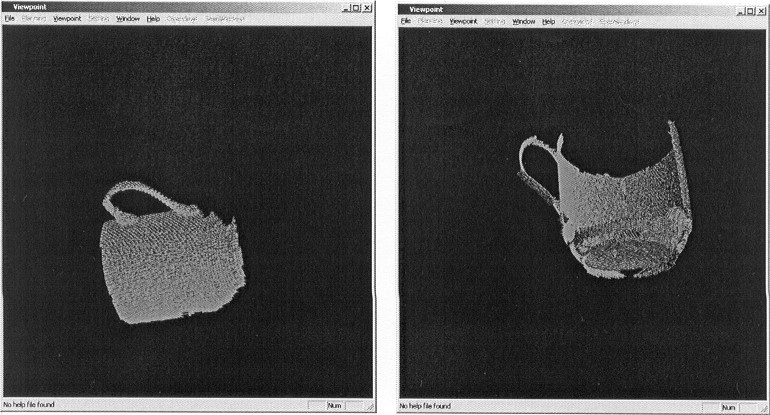
\includegraphics[scale=0.3]{PIC16}
		\caption{从第三视图中获得三维曲面,并与所有已知视图集成。}
		\label{fig-16}
	\end{figure}
	\begin{figure}[H]
		\centering
		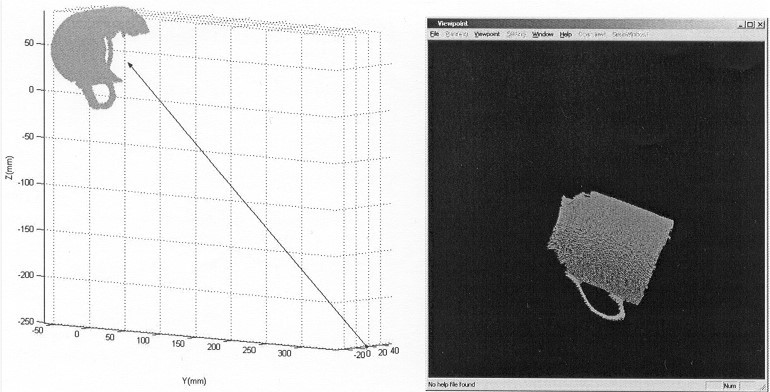
\includegraphics[scale=0.3]{PIC17}
		\caption{下一个视点和获得的三维曲面}
		\label{fig-17}
	\end{figure}

	最后,通过整合所有四个视图得到完整的模型。图\ref{fig-18}给出了它们与物体模型在三维空间的相对分布。此外,图\ref{fig-19}显示了另一个具有五个视点的物体。3-D动画的结果可以在我们的网站:http://vision.research.sychen.com/看到。在我们的实验中,是在一台750-MHz CPU的PC上实现的。三维表面采集是通过独特的颜色编码方法实现的。规划下一个视点的计算时间约为3-5秒,需要注意的是,规划结果取决于第一视点。由不同的初始视点,结果也是不同的,每个物体可能会多规划一到两个视点。
	\begin{figure}[H]
		\centering
		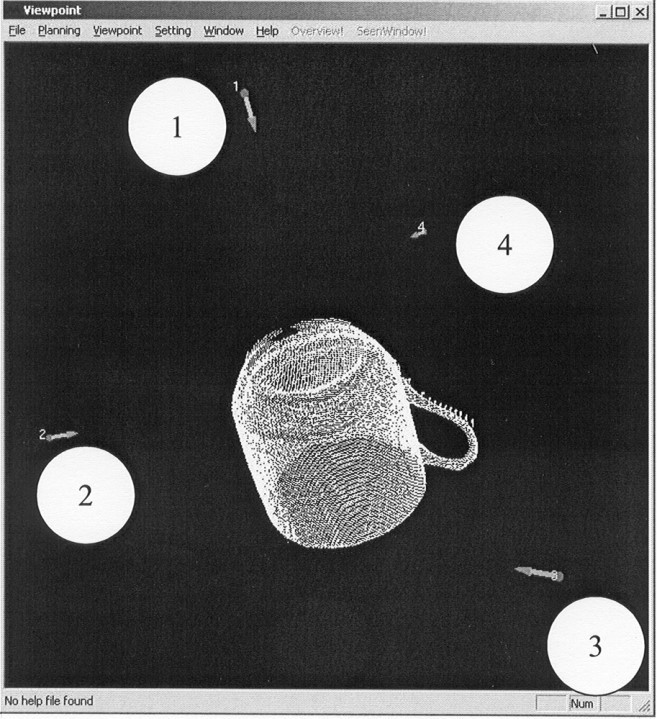
\includegraphics[scale=0.4]{PIC18}
		\caption{下一个视点和获得的三维曲面}
		\label{fig-18}
	\end{figure}
	\begin{figure}[H]
		\centering
		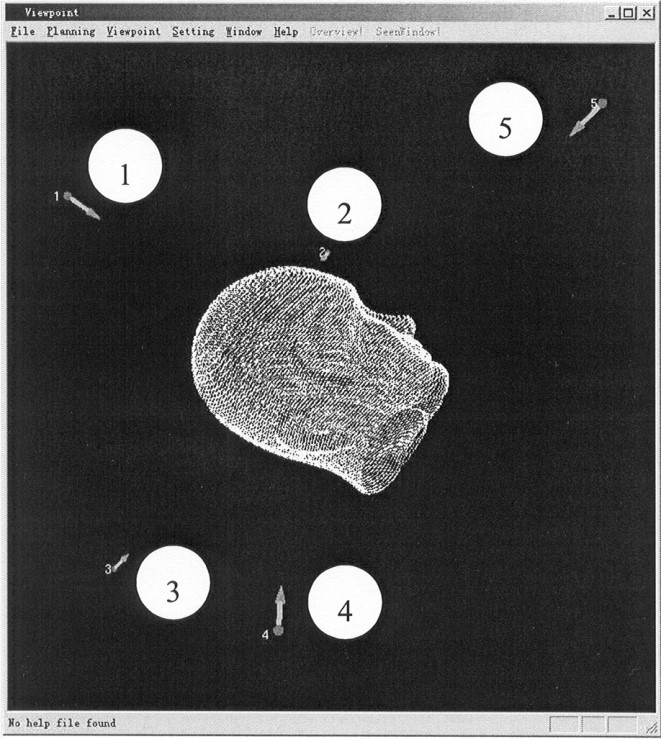
\includegraphics[scale=0.4]{PIC19}
		\caption{下一个视点和获得的三维曲面}
		\label{fig-19}
	\end{figure}

	\subsection{讨论}
	对于曲面边缘和物体边界,由于这些区域周围的曲率突然变化,在计算曲面趋势时将会有很大的误差。例如,如果有表面边缘位于所见区域,则确定常数$ a $和$ b $的已知部分的域应限制在一个不包含任何边缘的较小区域。还可能需要通过分析所见物体表面来改变勘探方向。
	
	当对一个小尺寸的物体建模时(与传感器的视场相比),趋势曲面法可能不是很好,因为整个物体将包含在一个单一的视图中,而且曲面趋势具有高阶。这使得预测未知区域变得不可靠。在这种情况下,可以采用基于传感器的解决方案\cite{pito1999solution}来代替目标驱动的方法来完成建模任务。
	
	本研究的基本思路是寻找任何可能的物体形状线索,用于预测未知区域。表面趋势是一种适合许多物体的选择。在这里,趋势可能不是由已知部分的所有面积来计算的,我们只选择合适的表面部分,通常没有物体的边界或边缘,这样的趋势是合理的和可预测的。例如,对于一个多面体物体,表面趋势将是一个单一的表面平面。只有当图像边界在多边形平面的边缘上时,才无法合理规划下一个视图。这种情况在实际中很少会发生。这样的问题也可以通过我们的选择勘探方向的方法来避免。当然,我们并不指望趋势法就能完成整个建模任务。我们需要将其与其他技术相结合,使整个建模过程以“自适应”的方式执行。需要注意的是,如果一个物体是简单的、光滑的,并且已知存在于有限的空间内(如一个球),可以采用规则的球体镶嵌法(如Zha\cite{zha1997active}的方法)来获取曲面,效率也差不多。但是,如果物体中含有任何偏离球面的不规则特征(如本文介绍的头部),常规的视点球面镶嵌法(半径固定)将无法提供任务所需的最优解。
	
	\section{结论}
	在本文中,我们提出了一种趋势面模型,用于预测物体或环境的未见部分。通过这种方式,可以确定下一个视点进行在线采集范围数据,直到重建物体或环境的整体结构。
	
	根据曲率趋势,计算出趋势面和趋势曲线。在确定下一个视角的同时,本文考虑了多个传感器放置的约束条件,如分辨率、视场角和视角。如果物体的未知曲面是由一阶和二阶曲线和曲面组成的,这样的趋势模型可以准确预测该曲面。已经完成的实验验证了本文提出的方法。
	
	在未来的研究工作中,我们将处理复杂的局部模型上的边界位置的可靠检测,以便对它们进行评估,以选择最佳的勘探方向的候选点。其他不确定的条件也将被考虑,以使重建过程更加可靠,从而使自主机器人系统可以在没有任何人类干扰的情况下工作。
	
	\nocite{*}
	\bibliography{scholar}
	
	\begin{flushright}
		\songti \zihao{4} \bfseries IEEE系统,人与控制论交易,B部分(网络论)(第35卷,发行:2005年10月5日)
	\end{flushright}

\end{document}
